% This file is for chapter 3
% This file is for chapter 3

\chapter{Parallel Portfolio Selection with Parallel Data Training}


\section{Introduction}

Combinatorial problem solvers often exhibit complementary performance when solving given problem instances. The use of algorithms portfolios has proven to be more effective than choosing the best single solver (SBS) averaged across all instances \cite{Huberman1997,GOMES200143}. Different portfolio approaches and designs are presented in the literature. Entire portfolios can be run in parallel or a single algorithm can be selected instance by instance using algorithm selection techniques. 

This selection-based approach is often addressed by training performance models using machine learning algorithms and instance features \cite{Kotthoff2014,10.1162/evco_a_00242}. One drawback of this approach is that since no machine learning model is perfect, the selections might be incorrect, and performance models might not always be able to select the best algorithm for a given instance. This means that selecting the wrong algorithm can waste time and resources. 

Since the hardware architecture of modern computing units can handle multiple tasks in parallel, another portfolio approach is to execute the entire portfolio simultaneously. This approach avoids the drawback of algorithm selection, as the actual best solver will always be included in the portfolio and executed alongside other algorithms. However, running too many solvers in parallel can lead to resource wastage by overloading computing processors. Additionally, this method can introduce significant overhead, as solvers and cores compete for shared resources when too many solvers are executed simultaneously. The more algorithms executed in parallel, the greater the risk of time-out computations and overhead. The preliminary results presented in Chapter 3 \cite{pmlr-v140-kashgarani21a} showed that, while the selection of a single algorithm is suboptimal and imperfect, it performs better than running too many solvers in parallel.

In Chapter 4, we proposed a hybrid approach that combines the benefits of algorithm selection and parallel execution. We further extend this method to a variation that performs competitively with the original approach in Chapter 5. These "middle-path" methods aim to select the most promising subset of algorithms to run in parallel on a single non-distributed computing node \cite{kashgarani2023automatic}. These promising methods optimized performance by utilizing regression-based random forest algorithm selectors, incorporating the estimated uncertainty of predictions, and accounting for the overhead associated with parallel portfolio execution. However, these approaches were tested using performance models trained on sequential data, which do not account for the overhead associated with parallel execution.

In this chapter, instead of relying on regression random forest models trained on sequential data, we train performance models using actual parallel data. We then compare algorithm selectors trained on sequential data with those trained on parallel data, applying the method proposed in Chapter 4 for parallel portfolio selection. By evaluating the effectiveness of these two types of algorithm selector in portfolio selection, we investigate whether collecting parallel data provides a significant advantage or whether sequential data are equally effective.

\section{Training Performance Modeling with Parallel Data}
In the paper Chapter 4 and 5\cite{kashgarani2023automatic}, we used data collected from running a single solver exclusively on a computing node to train the regression-based random forest model. This data does not account for parallelization or the overhead associated with running multiple solvers concurrently. Although this approach has proven effective, since we have already collected parallel data, we now aim to investigate the efficiency of training the performance model using these parallel data as well. Specifically, we focus on training performance models on parallel data. These parallel data are gathered by running solvers in parallel alongside other solvers, with varying numbers of solvers executed simultaneously on a single, exclusive computing node ensuring that no other tasks interfere with the recorded runtimes.

In this approach, for scenarios such as SAT11-NDU, SAT18-EXP, SAT16-MAIN, and IPC2018, where data are available for up to 10 parallel runs, we trained 10 distinct performance models, each tailored to a specific level of parallelization. Similarly, for MAXSAT2019, which includes data for up to 7 parallel runs, we trained 7 separate models, each trained for a given parallel run level. This means that the performance model, trained on data collected from running $n$ parallel runs, is used to predict the performance of a solver when running $n$ parallel runs. 

\subsection{Parallel Portfolio Selection}
Algorithm performance for combinatorial problems varies widely between instances, and portfolio approaches that use machine learning-based algorithm selection aim to optimize performance by selecting the best algorithms to execute while minimizing overhead from concurrent execution. Algorithm selection has been effective in domains like SAT and mixed integer programming. However, selecting a single algorithm can sometimes lead to suboptimal outcomes due to inaccurate predictions. This issue can be addressed by selecting a small subset of algorithms to run in parallel, which mitigates prediction inaccuracies while reducing overhead and resource demands.

We follow the methods and equations outlined in Chapter 4 as described in~\cite{kashgarani2023automatic}. We do not include the subportfolio selection method using KL divergence, as it consistently performed worse than the method proposed in Chapter 4. The selection approach in Chapter 4 aims to select a subportfolio of solvers to run in parallel for a given problem instance by leveraging predicted performance rankings. Solvers are ranked according to their predicted performance metric, forming a total order, and a subset of size $n$ is selected from the top-ranked solvers. The key challenge is determining the optimal portfolio size $n$, as including too many algorithms increases the chance of including the best solver but also introduces significant overhead from running solvers in parallel. To address this, the method incorporates a probabilistic approach using the predicted performance distribution of each solver.

Rather than relying on point predictions, the method uses the predicted performance distributions and extends typical algorithm selection practices by incorporating uncertainty of performance predictions. We assume that predictions follow a normal distribution characterized by their mean and standard deviation. The overlap between these distributions is used to compute the likelihood that a solver performs comparably to the best-predicted solver. A threshold parameter, $p_{\cap}$, controls the size of the parallel portfolio by including solvers whose distributions overlap sufficiently with that of the best solver. This approach balances the trade-off between including solvers that might achieve optimal performance and limiting computational overhead, providing a flexible and robust framework for parallel portfolio selection. 

As in previous chapters, we used regression random forests as the algorithm selector, identified as the best performing approach in the ASLib study \cite{BISCHL201641}. Furthermore, we transitioned from using a model trained exclusively on sequential data to one trained on sequential and parallel data to assess their comparative effectiveness. Through this approach and our experiments, we sought to optimize the utilization of parallel computational resources for solving combinatorial problems while minimizing the overhead associated with parallel execution.


\section{Experimental Setup}
\subsection{Data Collection}
We used the same five scenarios from previous chapters \cite{kashgarani2023automatic}, all now included in the ASlib benchmark repository \cite{BISCHL201641}: MAXSAT19-UCMS, SAT11-INDU, SAT18-EXP, SAT16-MAIN, and IPC2018. Although the ASlib data repository only provides performance data for single runs, we incorporated parallel run measurements from \cite{kashgarani2023automatic}, performed on standalone machines. For MAXSAT19-UCMS, SAT11-INDU, SAT16-MAIN, and SAT18-EXP, 54 features are computed using the SATZilla feature extraction code \cite{satzilla}. For IPC2018, feature extraction tool by \cite{Fawcett_Vallati_Hutter_Hoffmann_Hoos_Leyton-Brown_2014} generated 305 features. The scenarios, data and features of our experiments align with those used in \cite{kashgarani2023automatic}, as summarized in Table~\ref{tab:scenarios6}.

The data were collected on compute nodes with 32 processors, a 40 MB cache (Intel(R) Xeon(R) CPU E5-2683 v4 @ 2.10GHz), and 128 GB of memory, running Red Hat Linux version 8.6. We adhered to the ASlib time limits: 5000 CPU seconds for SAT18-EXP, SAT11-INDU, and SAT16-MAIN; 3600 seconds for MAXSAT19-UCMS; and 1800 seconds for IPC2018. Each algorithm was individually executed over 2 to 10 parallel runs during data collection.

\begin{table}
\centering
\caption{Number of Algorithms, Instances, and Features Across All Scenarios.}
\label{tab:scenarios6}
\begin{tabular}{p{5cm} cccc}
\toprule
Scenario & Algorithms & Instances & Instance Features\\
\midrule
IPC2018 & 15 & 240 & 305\\
MAXSAT19-UCMS & 7 & 572 & 54\\
SAT11-INDU & 14 & 300 & 54\\
SAT16-MAIN & 25 & 274 & 54\\
SAT18-EXP & 37 & 353 & 54\\
\bottomrule
\end{tabular}
\end{table}

\subsection{Training and Tuning}
We constructed random forest regression models using the Ranger implementation from the MLR3 package \cite{ranger} in R to predict the algorithm performance in specific instances. Although we previously presented results from various random forest implementations in R, this chapter focuses exclusively on Ranger models to compare the performance of models trained on sequential data with those trained on parallel data. Our setup closely follows the methodology outlined in Chapter 4 and in \cite{BISCHL201641}: we excluded instance features with constant values and imputed missing feature values using the mean of all nonmissing values for each feature. The random forest hyperparameters were optimized using random search with 250 iterations, varying $ntree$ between 10 and 200 and mtry between 1 and 30. Nested cross-validation with three inner folds and ten outer folds was used for model evaluation \cite{BISCHL201641}.

For training the models with parallel data, we trained 10 models for the SAT11-INDU, SAT16-MAIN, SAT18-EXP, and IPC2018 scenarios, and 7 models for the MAXSAT19-UCMS scenario, as only 7 solvers are available for this benchmark. Each model was trained using the runtimes associated with its specific parallel configuration. For instance, we trained one performance model using the runtimes of algorithms running in parallel with 2 other solvers, another model using the data collected when running 3 solvers in parallel, and so forth.

Our random forest regression models, built with the MLR3 and Ranger packages, predict solver runtime as the mean of the underlying distribution and estimate the standard deviation using the Jackknife and Infinitesimal Jackknife methods \cite{wager2014confidence, mlr}. The Jackknife method calculates the standard deviation of the mean predictions in all training observations. In this approach, the random forest model is trained on $n-1$ observations, leaving one out for prediction, and this process is repeated for each observation. The mean prediction for each tree is calculated by averaging its predictions for the left-out observations. The Jackknife method assumes a normal distribution of the predictions, where the standard deviation quantifies the uncertainty of the overall prediction. The Infinitesimal Jackknife method, rather than completely removing observations, assigns them a small weight to account for their influence on the model. 

The tuned $p_{\cap}$ values of Equation~\ref{eq:7} for each benchmark and model are provided in Table \ref{tab:pcap}. These values were individually optimized for each scenario to ensure that the selected portfolio achieved an optimal balance between performance and computational efficiency.

We first compare the predictions of the performance models trained on sequential data with those trained on data collected under different levels of parallelism. The analysis was performed using the McNemar test to assess whether there are significant differences in predictive performance between the sequential and parallel models in various scenarios. For each scenario, models trained on sequential data were compared with models trained on parallel data, involving varying numbers of parallel runs, ranging from 2 to the maximum number of solvers available for each scenario. We used contingency tables to capture the outcomes: instances where both models made correct or incorrect predictions and instances where one model succeeded while the other failed. The McNemar test provided p-values and test statistics for each comparison. The resulting $p-values$ indicate significant differences between the predictions of sequential and parallel models across all with significant level $\alpha = 0.05$ configurations. For example, in the MAXSAT2019 scenario, the $p-value$ for models trained with 2 parallel runs was $2.51e-8$, highlighting substantial differences in their predictions compared to sequential models. Similar trends were observed in other scenarios, such as IPC2018 and SAT18-EXP, where p-values remained very low at different levels of parallelism. These results demonstrate that the predictions of sequential models are notably distinct from those of parallel models, with significant differences observed in most scenarios and configurations.

Although the McNemar tests showed that the predictions are significantly different, we further investigated the Critical Difference (CD). CD analysis reveals that while the predictions of algorithm selectors trained in sequential and parallel data may vary, their ranking among the models on the five benchmarks is not significantly different at $\alpha = 0.05$. Using a critical difference value of 6.06 (calculated for 10 models and 5 datasets), the CD diagram in Figure~\ref{fig:critical} confirms that the variations in average ranks fall within the nonsignificant range. For instance, the average ranks of the models show minor differences across parallel configurations (e.g., the Sequential model has an average rank of 4.11 compared to the "10 parallel runs" model with 6.12), but these differences do not exceed the CD threshold. The rankings of the average ranks matrix in Table~\ref{tab:rank_mat} highlight consistent algorithm selection performance trends in datasets such as MAXSAT2019, IPC2018, SAT11-INDU, SAT16-MAIN and SAT18-EXP. Although individual rankings may differ slightly between scenarios, the overall rankings do not exhibit significant divergence. This suggests that algorithm selectors, whether trained in sequential or parallel data, produce models that rank algorithms similarly in terms of performance when evaluated across multiple datasets. 

\begin{table}[ht]
\centering
\caption[P-Values for McNemar Tests Comparing Models Trained on Parallel vs. Sequential Data]{P-values for McNemar tests comparing models trained on parallel data with the model trained on sequential data. The McNemar tests were conducted by selecting the top single solver based on the performance model and constructing the corresponding 2x2 contingency matrix.}\label{p-values-macnemar-infjack}
\label{tab:scenarios2}
\begin{tabular}{lccccc}
\hline
Model & \small{MAXSAT19-UCMS} & IPC2018 & SAT11-INDU & SAT16-MAIN & SAT18-EXP \\ 
\hline
% sequential & 1.00e+00 & 1.00e+00 & 1.00e+00 & 1.00e+00 & 1.00e+00 \\ 
2 parallel runs & 2.51e-08 & 3.39e-02 & 4.53e-03 & 4.54e-04 & 6.17e-04 \\ 
3 parallel runs & 2.19e-06 & 4.89e-03 & 2.85e-02 & 1.42e-03 & 2.29e-04 \\ 
4 parallel runs & 3.97e-04 & 9.51e-04 & 1.05e-03 & 1.26e-03 & 2.97e-04 \\ 
5 parallel runs & 3.15e-05 & 1.39e-03 & 5.66e-03 & 1.56e-03 & 7.66e-04 \\ 
6 parallel runs & 8.25e-04 & 5.85e-03 & 4.01e-03 & 9.37e-04 & 3.83e-04 \\ 
7 parallel runs & 3.80e-03 & 8.97e-03 & 3.68e-02 & 3.82e-03 & 6.14e-06 \\ 
8 parallel runs & -- & 4.65e-04 & 1.13e-03 & 1.76e-04 & 6.85e-06 \\ 
9 parallel runs & -- & 4.07e-04 & 4.67e-02 & 1.09e-03 & 1.28e-04 \\ 
10 parallel runs & -- & 2.16e-04 & 5.07e-03 & 1.09e-03 & 2.28e-05 \\ 
   \hline
\end{tabular}
\end{table}

\begin{table}[ht]
\centering
\caption{Ranking Matrix for Critical Difference}\label{tab:rank_mat}
\small
\setlength{\tabcolsep}{4pt} % Reduce column spacing
\renewcommand{\arraystretch}{1.1} % Adjust row spacing
\begin{tabular}{lcccccccccc}
  \hline
 & \textbf{Seq.} & \textbf{2p} & \textbf{3p} & \textbf{4p} & \textbf{5p} & \textbf{6p} & \textbf{7p} & \textbf{8p} & \textbf{9p} & \textbf{10p} \\ 
  \hline
MAXSAT19-UCMS & 3.42 & 3.65 & 4.01 & 3.92 & 4.21 & 4.42 & 4.38 & -- & -- & -- \\ 
IPC2018 & 3.88 & 4.59 & 4.94 & 5.19 & 5.28 & 5.96 & 5.69 & 6.19 & 6.58 & 6.69 \\ 
SAT11-INDU & 4.18 & 4.58 & 4.67 & 5.25 & 5.28 & 5.83 & 5.88 & 6.34 & 6.32 & 6.68 \\ 
SAT16-MAIN & 5.13 & 4.98 & 4.85 & 5.07 & 5.42 & 5.53 & 5.61 & 5.77 & 6.51 & 6.13 \\ 
SAT18-EXP & 3.94 & 4.80 & 5.11 & 5.61 & 5.55 & 6.01 & 6.17 & 6.44 & 6.40 & 4.99 \\ 
\hline
\textbf{Average} & 4.11 & 4.52 & 4.71 & 5.01 & 5.15 & 5.55 & 5.54 & 6.19 & 6.45 & 6.12 \\   
\hline
\end{tabular}
\end{table}

\begin{figure}
        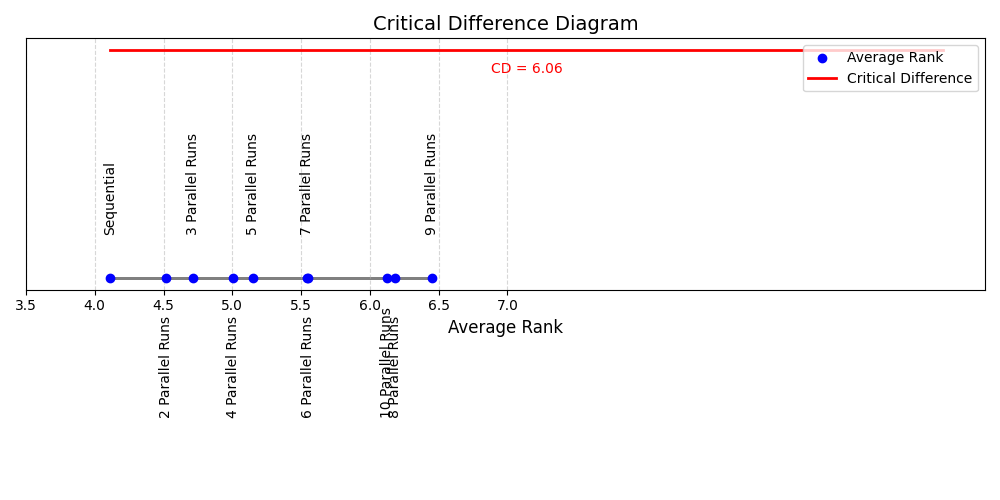
\includegraphics[width=.8\linewidth]{plots/Alternating_Label_Critical_Difference_Diagram.png}
    \caption[Critical Difference Diagram: Rankings of Performance Models Trained on Sequential vs. Parallel Data]{Critical Difference Diagram. This figure shows the average ranking of each performance model trained at different levels of parallelism, based on the actual performance of the selected algorithms. The CD of 6.06 means that the Critical Difference (CD) threshold for determining statistically significant differences in rankings is 6.06. If the difference in average rankings between two models is greater than 6.06, the rankings are considered statistically significantly different at a significance level of $\alpha=0.05$.}
    \label{fig:critical}
\end{figure}

\subsection{Baselines}

Although the algorithm selection rankings did not show significant differences in algorithm selection in these five scenarios, we evaluated the performance of the dynamic parallel portfolio approach against several baseline methods using sequential and parallel data-trained models. Specifically, we compared the results to the sequential Virtual Best Solver (VBS), which selects the best solver for each problem instance with a cumulative misclassification penalty of zero, and the sequential Single Best Solver (SBS), which is the solver with the best average performance across all instances and has a cumulative misclassification penalty of one. For parallel runs, the VBS selects the best solver for each instance but accounts for the overhead of $n$ parallel runs. The parallel SBS is determined similarly, based on the solver with the best average performance across all instances instead of the best solver for each instance. To ensure a realistic evaluation, we executed multiple solvers in parallel to measure the actual runtime of the best solver in this setup, rather than assuming it would run sequentially.

We used two methods to train algorithm selectors: one trained using Ranger with the Jackknife method and another using Ranger with the Infinitesimal Jackknife method to estimate the uncertainty of predictions. Initially, we trained models on sequential data and then trained performance models on parallel performance data ($AS_{\parallel}$). In the $AS_{\parallel}$ method, to predict performance for $n$ parallel runs, we used the predictions of the performance model trained on data collected from $n$ parallel runs.

We evaluated the proposed approach using three metrics: penalized average runtime with a factor of 10 (PAR10), misclassification penalty (MCP), and runtime. The PAR10 metric corresponds to the actual runtime if the algorithm successfully solves the instance within the timeout; otherwise, it is calculated as the timeout multiplied by 10. The MCP represents the difference between the performance of the selected algorithm and that of the optimal algorithm. To ensure comparability across scenarios, all performance metrics are normalized relative to the Virtual Best Solver (VBS) and Single Best Solver (SBS). The results, shown in Figure~\ref{fig:parallelvssequential}, depict the proportion of the performance gap closed by each approach. On this normalized scale, a value of 0 corresponds to the performance of the SBS, while a value of 1 corresponds to the performance of the VBS.

\section{Results}

We experimented with training Ranger models using parallel data to compare their performance with models trained on sequential data. Figures~\ref{fig:rangervsrf} present the PAR10 score results in terms of the normalized performance gap between the sequential Single Best Solver (SBS) and the sequential Virtual Best Solver (VBS) across all scenarios and processor counts. These figures specifically compare Ranger models trained with the Infinitesimal Jackknife method. Additionally, Tables~\ref{tab:summary6-ipc-max},~\ref{tab:summary6-sat11-sat16} and~\ref{tab:summary6-sat18} provide the exact runtime, Misclassification Penalty (MCP), and PAR10 scores for the methods, limiting the maximum number of parallel runs to 10 for SAT18-EXP, SAT16-MAIN, SAT11-INDU, and IPC2018, and to 7 for MAXSAT19-UCMS.

\begin{figure}[ht]
        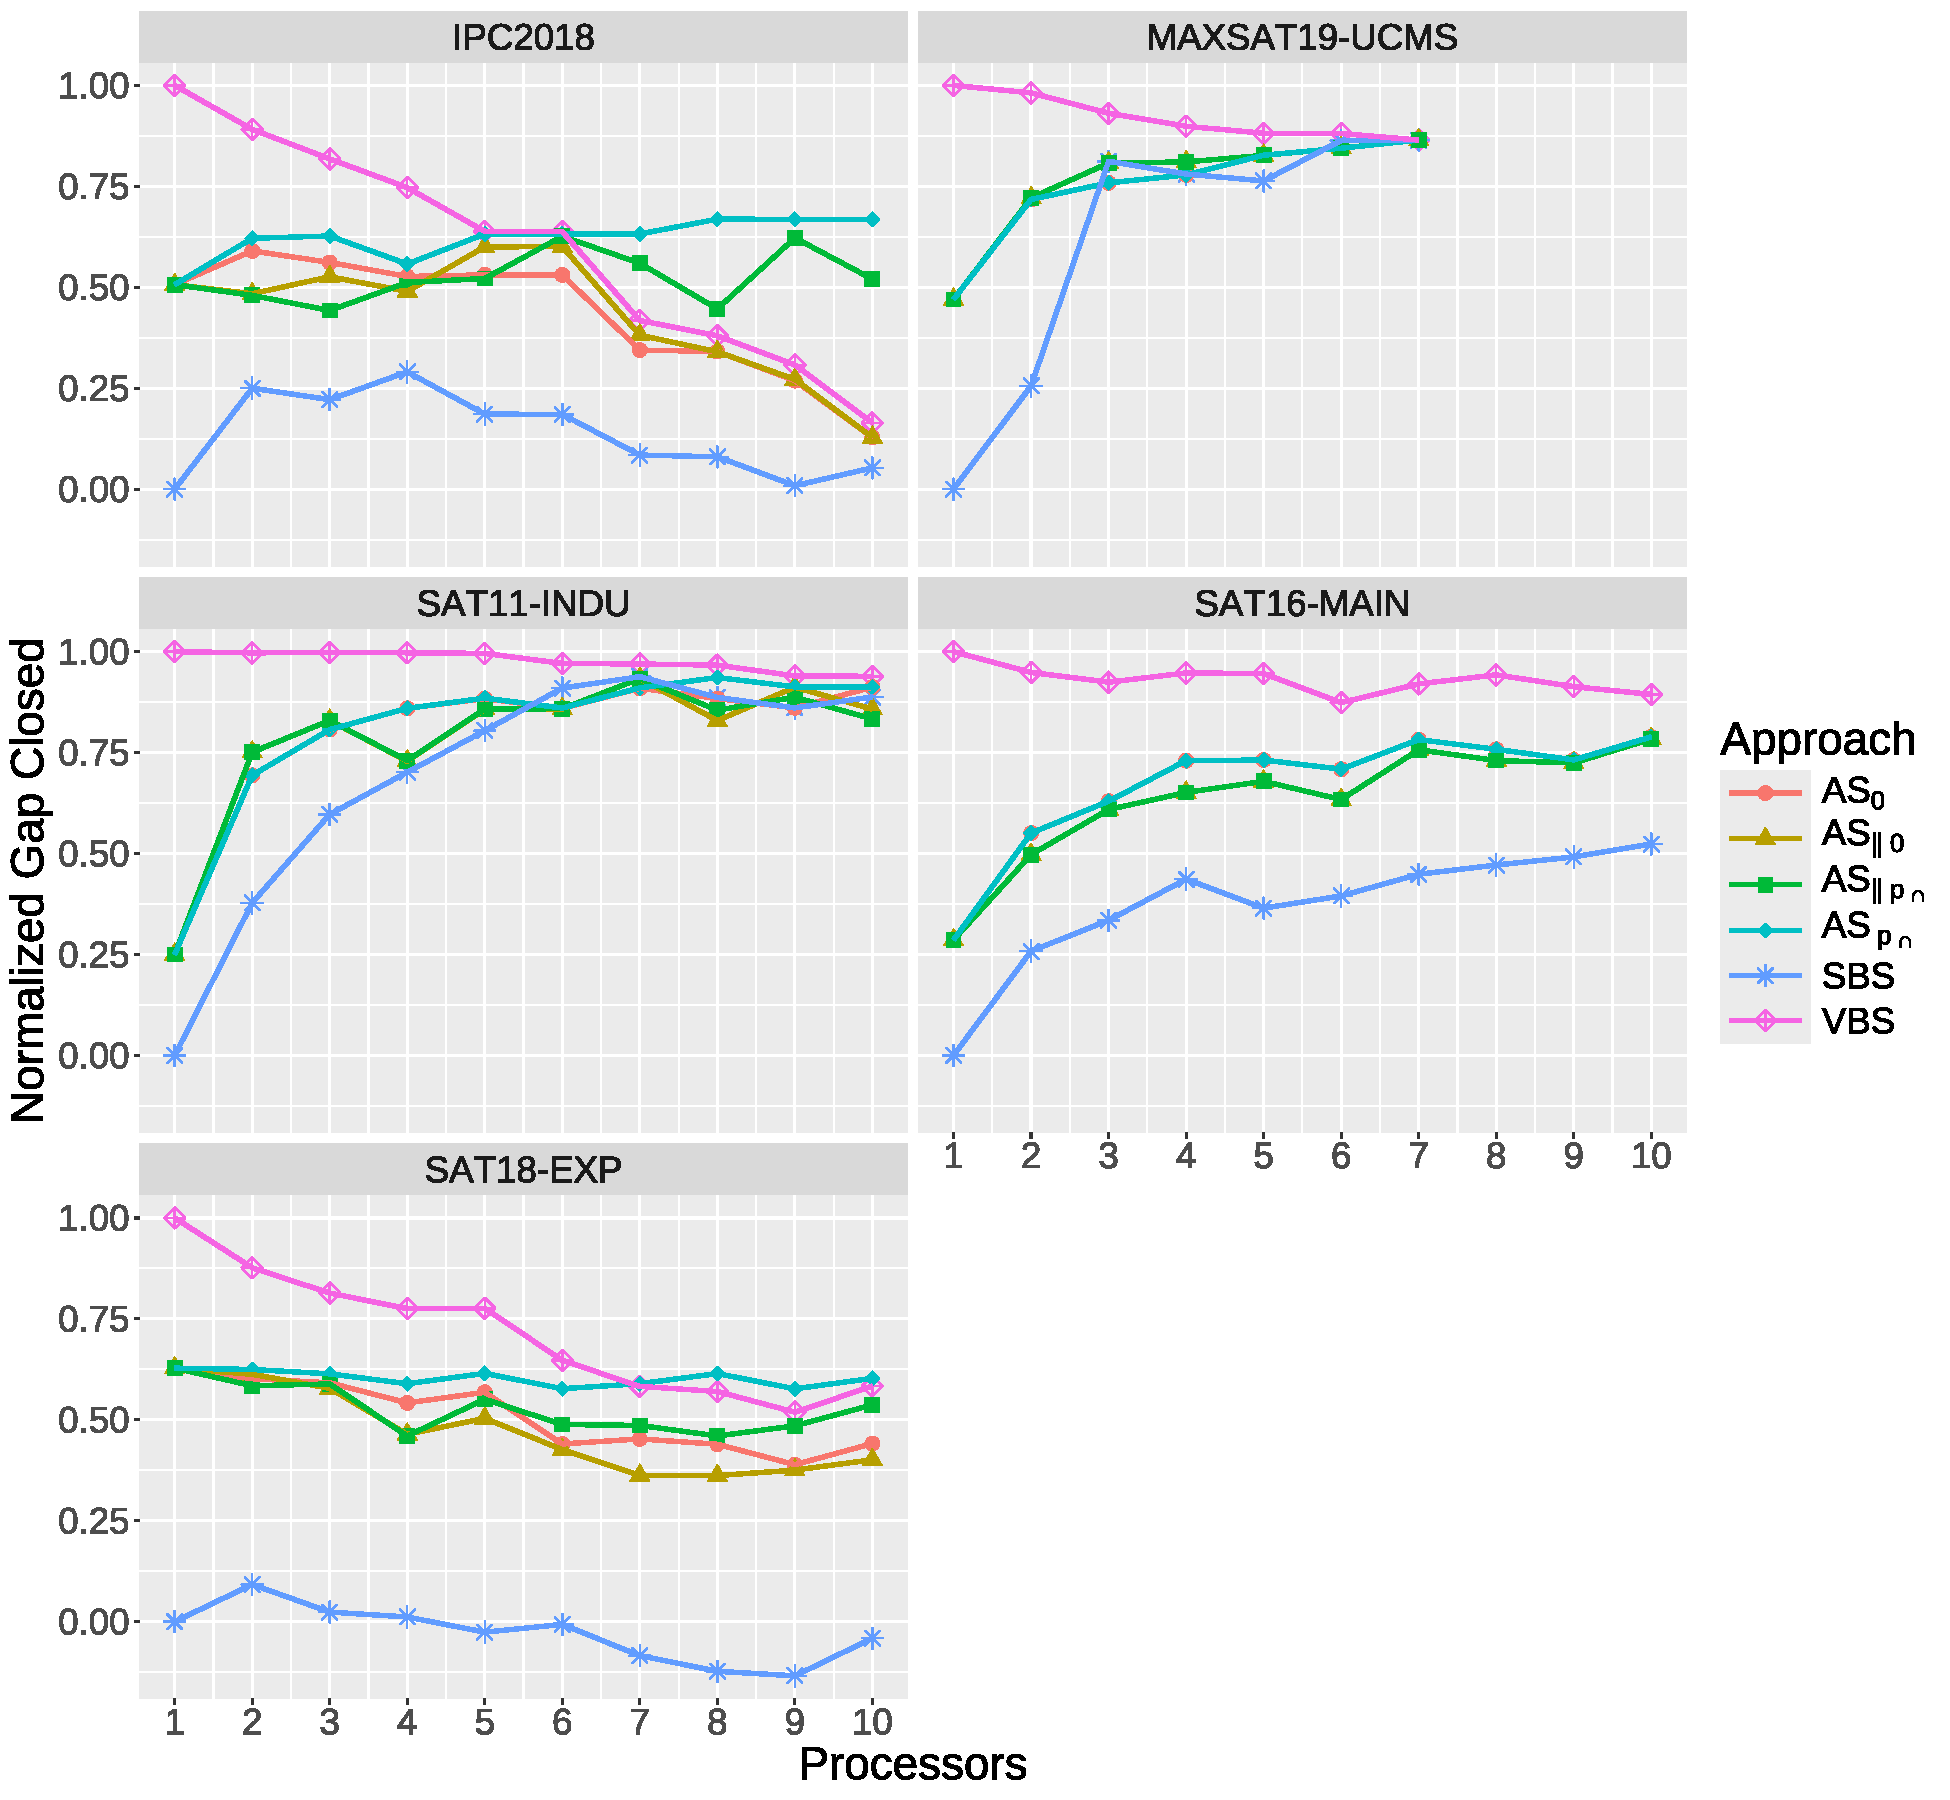
\includegraphics[width=\linewidth]{plots/pl_pcap_comparison_line_chart_parallel_NormalizedGap.pdf}    
    \caption[Results Summary: Comparing $AS_{p_{\cap}}$ with $AS_{\parallel p_{\cap}}$ Performance]{
    Results Overview. The plot illustrates the extent to which each method narrows the gap between the PAR10 scores of the Single Best Solver (SBS) and the Virtual Best Solver (VBS). For VBS and SBS, the top $n$ solvers are selected, where $n$ matches the number of processors available for each problem instance and across all instances, respectively. $AS_0$ selects the top $n$ solvers as predicted by algorithm selection, disregarding any overlap in their predicted runtime distributions. $AS_{p_{\cap}}$ follows the approach proposed in \cite{kashgarani2023automatic}, with the number of processors capped at the specific value on the x-axis — fewer solvers than this maximum may be selected based on the overlap in runtime predictions. The algorithm selection here is Ranger model with the Infinitesimal Jackknife method for predicting uncertainty. The $\parallel$ symbol is referring to the performance model trained on parallel data.
    }
    \label{fig:parallelvssequential}
\end{figure}


\begin{table}
\begin{center}
    {\caption[Detailed Results: Runtime, MCP, PAR10, and Normalized Gap Closed for $AS_{p_{\cap}}$ vs. $AS_{\parallel p_{\cap}}$ for IPC2018 and MAXSAT19-UCMS Scenarios]{Detailed results. Mean and standard deviation of values for runtime, MCP, and PAR10 across all problem instances in a scenario for the sequential virtual best solver, sequential single best solver, and single top predicted algorithm in the initial three rows. The second set of rows for each scenario shows the results for the maximum number of processors (10 for IPC2018, and 7 for MAXSAT19-UCMS) for our approaches and the baselines we compare to. All numbers were rounded to integers. The best value for each scenario and measure is shown in \textbf{bold} (excepting the sequential VBS, which is by definition always the best), the second best in \textit{italics}. The normalized gap closed represents the mean and standard deviation of the normalized gap closed across the folds.}\label{tab:summary6-ipc-max}}
    \scriptsize\begin{tabular}{clcccc}
    \toprule
        Scenario & Approach & Runtime [s] & MCP & PAR10 & NormalizedGap\\
    \midrule
    
    \multirow{17}{*}{\rotatebox{90}{IPC2018}} & \multicolumn{5}{c}{\textbf{1 Processor}} \\\cmidrule{2-6}
        & VBS & 508$\pm$697 & 0 & 3478$\pm$6903 & 1\\
        & AS (RI) & 608$\pm$751 & 100$\pm$293 & 4456$\pm$7583 & -0.35$\pm$2.85\\
        & AS (RJ) & 604$\pm$752 & 96$\pm$293 & 4519$\pm$7633 & -0.39$\pm$2.84 \\
        & SBS & 734$\pm$770 & 226$\pm$414 & 5459$\pm$8072 & 0 \\
    \cmidrule{2-6}  
    & \multicolumn{5}{c}{\textbf{10 Processors}}\\
    \cmidrule{2-6}
        & $AS_0$ (RI)  & 616$\pm$783  & 107$\pm$312 & 5206$\pm$8065 & -0.69$\pm$2.54\\
        & $AS_0$ (RJ)  & 616$\pm$783 & 107$\pm$312 & 5206$\pm$8065 & -0.69$\pm$2.54 \\ 
        & $AS_{p_{\cap} = 0.44}$ (RI) & \textbf{557$\pm$728} & \textbf{49$\pm$190} & \textbf{4135$\pm$7403} & \textbf{-0.19$\pm$2.89}\\
        & $AS_{p_{\cap} = 0.27}$ (RJ) & 570$\pm$744 & \emph{62$\pm$229} & 4350$\pm$7552 &  \emph{-0.21$\pm$2.72} \\
        & $AS_{\parallel 0} (RI) $ & 615$\pm$782 & 107$\pm$311 & 5205$\pm$8065 & -0.69$\pm$2.55\\
        & $AS_{\parallel 0} (RJ) $ & 619$\pm$786 & 112$\pm$322 & 5277$\pm$8102 & -0.71$\pm$2.54\\ 
        & $AS_{\parallel p_{\cap} = 0.44} (RI) $ & 581$\pm$743 & 73$\pm$252 & 4428$\pm$7596 & -0.34$\pm$2.67\\
        & $AS_{\parallel p_{\cap} = 0.27} (RJ) $ & 608$\pm$771 & 100$\pm$304 & 4996$\pm$7946 & -1.5$\pm$5.65\\ 

    \midrule
    \multirow{19}{*}{\rotatebox{90}{MAXSAT19-UCMS}} & \multicolumn{5}{c}{\textbf{1 Processor}} \\\cmidrule{2-6}
        & VBS & 858$\pm$1476 & 0 & 7768$\pm$14717 & 1\\
        & AS (RI) & 1076$\pm$1575 & 218$\pm$729 & 9686$\pm$15850 & 0.45$\pm$0.34 \\
        & AS (RJ) & 1044$\pm$1565 & 186$\pm$666 & 9540$\pm$15793 & 0.49$\pm$0.23 \\
        & SBS & 1190$\pm$1657 & 332$\pm$940 & 11386$\pm$16696 & 0 \\
    \cmidrule{2-6}   
    & \multicolumn{5}{c}{\textbf{7 Processors}}\\
    \cmidrule{2-6}  
        & $AS_0$ (RI) & \textbf{894$\pm$1506} & \textbf{37$\pm$247} & \emph{8258$\pm$15062} & \emph{0.85$\pm$0.16} \\ 
        & $AS_0$ (RJ) & \textbf{894$\pm$1506} & \textbf{37$\pm$247} & \emph{8258$\pm$15062} & \emph{0.85$\pm$0.16}\\
        & $AS_{p_{\cap} = 0.03}$ (RI) & \textbf{894$\pm$1506} & \textbf{37$\pm$247} & \emph{8258$\pm$15062} & \emph{0.85$\pm$0.16}  \\ 
        & $AS_{p_{\cap} = 0.14}$ (RJ) & 921$\pm$1521 & 63$\pm$369 & 8568$\pm$15263 &  0.76$\pm$0.24 \\
        & $AS_{\parallel 0} (RI) $ & \textbf{894$\pm$1506} & \textbf{37$\pm$247} & \emph{8258$\pm$15062} & \emph{0.85$\pm$0.16}\\
        & $AS_{\parallel 0} (RJ) $ & \textbf{894$\pm$1506} & \textbf{37$\pm$247} & \emph{8258$\pm$15062} & \emph{0.85$\pm$0.16}\\
        & $AS_{\parallel p_{\cap} = 0.03} (RI) $ & \textbf{894$\pm$1506} & \textbf{37$\pm$247} & \emph{8258$\pm$15062} & \emph{0.85$\pm$0.16}\\
        & $AS_{\parallel p_{\cap} = 0.14} (RJ) $ & 939$\pm$1534 & 82$\pm$442 & 8756$\pm$15379 & 0.71$\pm$0.31\\

\bottomrule
    
    \end{tabular}    
\end{center}
\end{table}

\begin{table}
\begin{center}
    {\caption[Detailed Results: Runtime, MCP, PAR10, and Normalized Gap Closed for $AS_{p_{\cap}}$ vs. $AS_{\parallel p_{\cap}}$ for SAT11-INDU and SAT16-MAIN Scenarios]{Detailed results. Mean and standard deviation of values for runtime, MCP, and PAR10 across all problem instances in a scenario for the sequential virtual best solver, sequential single best solver, and single top predicted algorithm in the initial three rows. The second set of rows for each scenario shows the results for the maximum number of processors (10 for SAT16-MAIN and SAT11-INDU) for our approaches and the baselines we compare to. All numbers were rounded to integers. The best value for each scenario and measure is shown in \textbf{bold} (excepting the sequential VBS, which is by definition always the best), the second best in \textit{italics}. The normalized gap closed represents the mean and standard deviation of the normalized gap closed across the folds.}\label{tab:summary6-sat11-sat16}}
    \scriptsize\begin{tabular}{clcccc}
    \toprule
        Scenario & Approach & Runtime [s] & MCP & PAR10 & NormalizedGap\\
    \midrule
    \multirow{17}{*}{\rotatebox{90}{SAT11-INDU}} & \multicolumn{5}{c}{\textbf{1 Processor}} \\\cmidrule{2-6}
        & VBS & 1140$\pm$1836 & 0 & 8040$\pm$17905 & 1\\
        & AS (RI) & 1610$\pm$2108 & 470$\pm$1145 & 12710$\pm$21389 & -0.06$\pm$0.9\\
        & AS (RJ) & 1565$\pm$2049 & 425$\pm$1017 & 11315$\pm$20402 & 0.34$\pm$0.49\\
        & SBS & 1818$\pm$2168 & 678$\pm$1340 & 14268$\pm$22154 & 0 \\
    \cmidrule{2-6}    
    & \multicolumn{5}{c}{\textbf{10 Processors}}\\
    \cmidrule{2-6}    
        & $AS_0$ (RI) & \emph{1238$\pm$1892} & \emph{127$\pm$385} & \emph{8588$\pm$18350} & \textbf{0.92$\pm$0.1}\\ 
        & $AS_0$ (RJ) & 1262$\pm$1910 & 151$\pm$480 & 8612$\pm$18342 & \textbf{0.92$\pm$0.1} \\
        & $AS_{p_{\cap} = 0.01}$ (RI) & \textbf{1236$\pm$1890} & \textbf{121$\pm$379} & \textbf{8586$\pm$18351} & \textbf{0.92$\pm$0.1} \\ 
        & $AS_{p_{\cap} = 0.31}$ (RJ) & 1289$\pm$1934 & 178$\pm$595 & 9089$\pm$18787 & 0.78$\pm$0.28\\
        & $AS_{\parallel 0} (RI) $ & 1276$\pm$1926 & 166$\pm$546 & 8926$\pm$18643 & 0.89$\pm$0.13\\
        & $AS_{\parallel 0} (RJ) $ & 1286$\pm$1939 & 175$\pm$564 & 8936$\pm$18640 & 0.88$\pm$0.12\\
        & $AS_{\parallel p_{\cap} = 0.01} (RI) $ & 1279$\pm$1929 & 162$\pm$530 & 9079$\pm$18791 & 0.78$\pm$0.27\\
        & $AS_{\parallel p_{\cap} = 0.31} (RJ) $ & 1365$\pm$2004 & 247$\pm$794 & 10065$\pm$19605 & 0.64$\pm$0.24\\

   \midrule 
    \multirow{19}{*}{\rotatebox{90}{SAT16-MAIN}} & \multicolumn{5}{c}{\textbf{1 Processor}} \\\cmidrule{2-6}
        & VBS & 1867$\pm$2193 & 0 & 15005$\pm$22530 & 1\\
        & AS (RI) & 2383$\pm$2294 & 516$\pm$1151 & 19956$\pm$24111 & 0.05$\pm$0.66\\ 
        & AS (RJ) & 2400$\pm$2269 & 533$\pm$1177 & 19316$\pm$23880 & 0.3$\pm$0.24\\ 
        & SBS & 2560$\pm$2294 & 693$\pm$1415 & 21940$\pm$24464 & 0\\
    \cmidrule{2-6}
    & \multicolumn{5}{c}{\textbf{10 Processors}}\\
    \cmidrule{2-6}
        & $AS_0$ (RI)& \textbf{2016$\pm$2225} & \textbf{150$\pm$503} & \emph{16469$\pm$23122} & 0.68$\pm$0.6\\ 
        & $AS_0$ (RJ)& 2048$\pm$2228 & 181$\pm$597 & \textbf{16336$\pm$23023} & 0.68$\pm$0.59\\ 
        & $AS_{p_{\cap} = 0}$ (RI) & \textbf{2016$\pm$2225} & \textbf{150$\pm$503} & \emph{16469$\pm$23122} & 0.68$\pm$0.6\\ 
        & $AS_{p_{\cap} = 0.33}$ (RJ) & 2088$\pm$2239 & 222$\pm$704  & 16705$\pm$23156 & 0.64$\pm$0.37\\ 
        & $AS_{\parallel 0} (RI) $ & 2053$\pm$2246 & 186$\pm$593 & 16505$\pm$23101 & \emph{0.79$\pm$0.49} \\
        & $AS_{\parallel 0} (RJ) $ & \emph{2040$\pm$2223} & \emph{174$\pm$579} & 16000$\pm$22864 & \textbf{0.8$\pm$0.34} \\
        & $AS_{\parallel p_{\cap} = 0} (RI) $ & 2053$\pm$2246 & 186$\pm$593 & 16505$\pm$23101 & \emph{0.79$\pm$0.49} \\
        & $AS_{\parallel p_{\cap} = 0.33} (RJ) $ & 2197$\pm$2271 & 330$\pm$924 & 17635$\pm$23454 & 0.6$\pm$0.43\\

\bottomrule
    
    \end{tabular}    
\end{center}
\end{table}

\begin{table}
\begin{center}
    {\caption[Detailed Results: Runtime, MCP, PAR10, and Normalized Gap Closed for $AS_{p_{\cap}}$ vs. $AS_{\parallel p_{\cap}}$ for SAT18-EXP Scenario]{Detailed results. Mean and standard deviation of values for runtime, MCP, and PAR10 across all problem instances in a scenario for the sequential virtual best solver, sequential single best solver, and single top predicted algorithm in the initial three rows. The second set of rows for each scenario shows the results for the maximum number of processors (10 for SAT18-EXP) for our approaches and the baselines we compare to. All numbers were rounded to integers. The best value for each scenario and measure is shown in \textbf{bold} (excepting the sequential VBS, which is by definition always the best), the second best in \textit{italics}. The normalized gap closed represents the mean and standard deviation of the normalized gap closed across the folds.}\label{tab:summary6-sat18}}
    \scriptsize\begin{tabular}{clcccc}
    \toprule
        Scenario & Approach & Runtime [s] & MCP & PAR10 & NormalizedGap\\
    \midrule    
    \multirow{19}{*}{\rotatebox{90}{SAT18-EXP }} & \multicolumn{5}{c}{\textbf{1 Processor}} \\\cmidrule{2-6}
         & VBS & 1146$\pm$1945 & 0 & 9687$\pm$19547 & 1\\
         & AS (RI) & 1648$\pm$2151 & 502$\pm$1256 & 13758$\pm$22034 & 0.59$\pm$0.18\\
         & AS (RJ) & 1690$\pm$2170 & 543$\pm$1302 & 14183$\pm$22247 & 0.57$\pm$0.16\\
         & SBS & 2400$\pm$2249 & 1254$\pm$1832 & 20629$\pm$24280 & 0\\
    \cmidrule{2-6}    
    & \multicolumn{5}{c}{\textbf{10 Processors}}\\
    \cmidrule{2-6}    
         & $AS_0$ (RI) & 1654$\pm$2285 & 511$\pm$1324 & 15804$\pm$23194 & 0.42$\pm$0.29\\
         & $AS_0$ (RJ) & 1678$\pm$2288 & 535$\pm$1351 & 15956$\pm$23243 & 0.4$\pm$0.3 \\
         & $AS_{p_{\cap} = 0.55}$ (RI) & \textbf{1541$\pm$2191} & \textbf{397$\pm$1177} & \textbf{14034$\pm$22332} & \textbf{0.6$\pm$0.21}\\ 
         & $AS_{p_{\cap} = 0.58}$ (RJ) & 1622$\pm$2237 & 477$\pm$1268 & 15008$\pm$22805 & 0.5$\pm$0.25\\
         & $AS_{\parallel 0} (RI) $ & 1709$\pm$2303 & 566$\pm$1397 & 16242$\pm$23351 & 0.4$\pm$0.21\\
         & $AS_{\parallel 0} (RJ) $ & 1676$\pm$2294 & 533$\pm$1358 & 15954$\pm$23245 & 0.42$\pm$0.22\\
         & $AS_{\parallel p_{\cap} = 0.55} (RI) $ & 1624$\pm$2217 & 478$\pm$1218 & 14754$\pm$22660 & 0.54$\pm$0.2\\
         & $AS_{\parallel p_{\cap} = 0.58} (RJ) $ & 1708$\pm$2269 & 563$\pm$1363 & 15730$\pm$23095 & 0.43$\pm$0.25\\

    \bottomrule
    
    \end{tabular}    
\end{center}
\end{table}

\begin{figure}
    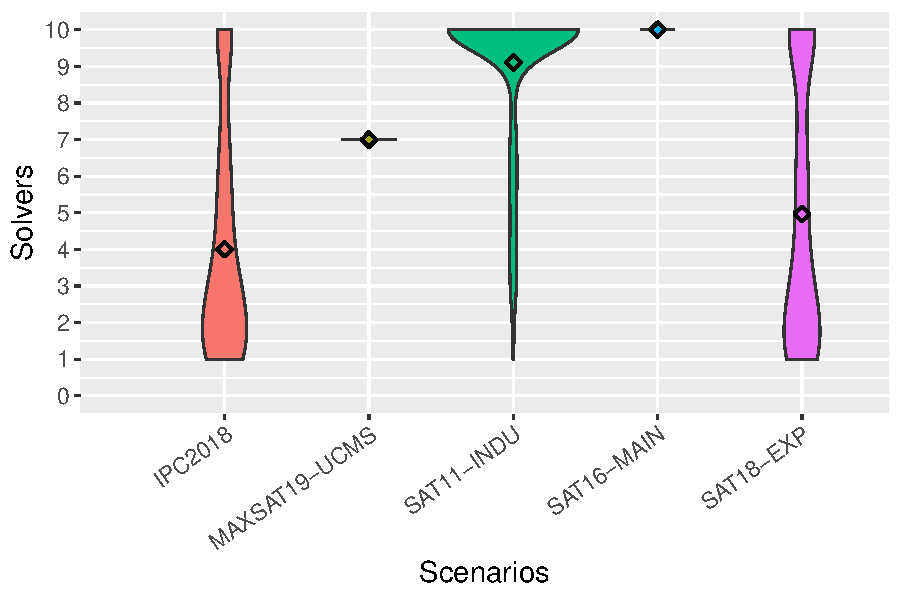
\includegraphics[width=0.5\linewidth]{plots/number_of_solvers_infjack_pcap_parallel.pdf}
    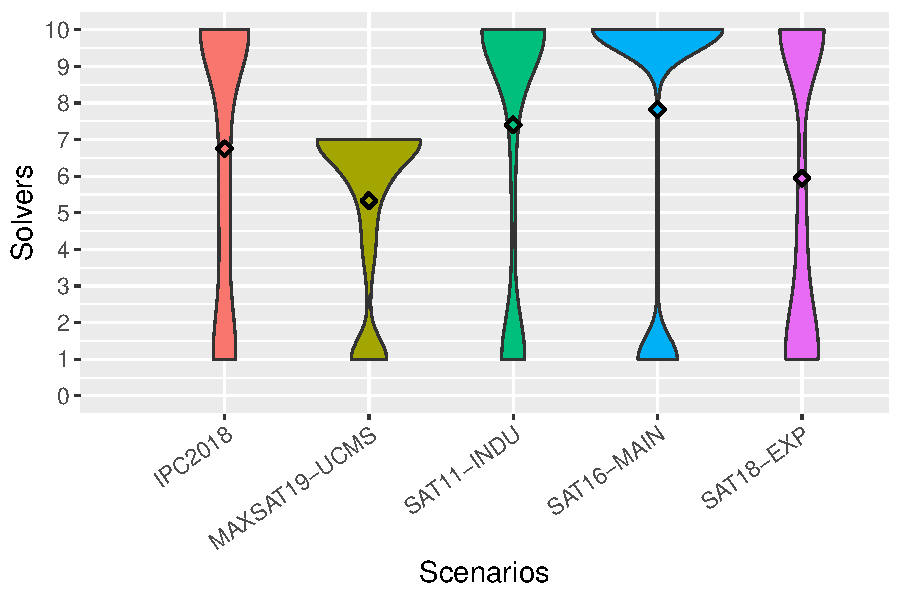
\includegraphics[width=0.5\linewidth]{plots/number_of_solvers_jack_pcap_parallel.pdf}

    \caption[Distribution of Number of Selected Solvers when Using $AS_{\parallel p_{\cap}}$]{
    Violin plot of the distribution of the number of selected solvers to run in parallel across all problem instances for each scenario for the respective optimal $p_{\cap}$ and the maximum level of parallelism (seven processors for MAXSAT19-UCMS and 10 for all other scenarios). The diamond denotes the mean value. The top-left plot refers to the RFJ model, the top-right plot to the RI model, and the bottom plot to the RJ model.
    }
    \label{fig:numberofsolvers_kl}
\end{figure}

When comparing models trained on sequential data with those trained on parallel data for portfolio selection, the model trained on sequential data consistently outperforms the model trained on parallel data. This is evident in Tables~\ref{tab:summary5-ipc-max}, \ref{tab:summary5-sat11-sat16} and~\ref{tab:summary5-sat18}, which show that both the $AS_0$ and $AS_{p_{\cap}}$ methods are superior to $AS_{\parallel 0}$ and $AS_{\parallel p_{\cap}}$, respectively. This holds for both the RJ and RI models in all scenarios, except when comparing $AS_0$ and $AS_{\parallel 0}$ for SAT16-MAIN and SAT18-EXP, where the RJ model performs slightly better. In Figure~\ref{fig:parallelvssequential}, for the RI model with a number of parallel runs limited to 10, the $AS_{\cap}$ method, using a model trained on sequential data, emerges as the best approach to portfolio selection.


\section{Conclusions}
In this chapter, we explore the impact of training algorithm selectors using parallel data versus sequential data for parallel portfolio selection. Using both sequential and parallel performance models, our objective was to understand whether incorporating data collected under parallel execution conditions would offer a significant advantage in portfolio selection tasks. Our initial analysis reveals that while predictions of algorithm selectors trained on parallel data differ significantly from those trained on sequential data, their overall rankings across models on the benchmarks are not significantly different. 

Furthermore, when comparing the effectiveness of portfolio selection, models trained on sequential data consistently outperform those trained on parallel data in most scenarios. Specifically, the $AS_{p_{\cap}}$ method trained in sequential data demonstrated superior performance compared to its counterpart trained in parallel data $AS_{\parallel p_{\cap}}$). 

These findings underscore the robustness of sequentially trained models for portfolio selection, even in parallel execution environments. Importantly, the results suggest that collecting parallel data may not be necessary for effective portfolio selection. Sequential data models are just as effective, if not superior, for predicting solver performance and guiding efficient portfolio selection. Although parallel data offers insight into runtime overheads, sequential data models remain more effective in predicting solver performance and ranking which resulted in efficient portfolio selection. 

% Cheat to bring in other references
%\nocite{*} % delete or comment this out.
